%=============================================================================
\documentclass[12pt]{article}
\usepackage{latexsym}
\usepackage{graphicx}
\usepackage{booktabs}
\usepackage{amsfonts}
\usepackage{amsmath}
\usepackage[caption=false]{subfig}
\usepackage{enumerate}
\usepackage{wrapfig}
%=============================================================================
\setlength{\evensidemargin}{-0.25in} 
\setlength{\oddsidemargin} {-0.25in}
\setlength{\textwidth}     {+7.00in}
\setlength{\topmargin}     {+0.00in}
\setlength{\textheight}    {+8.50in}
%=============================================================================
\makeatletter
\renewcommand{\baselinestretch}{1.2}
\newcommand{\ro}{R}
\normalsize
%=============================================================================

%==============================================================================
\pagestyle{plain}
%
\date{}
\begin{document}
	%==============================================================================
	\begin{flushleft}
		\large \bf
		Homework 10 \\
	\end{flushleft}
	%==============================================================================
{\bf
Please note that handwritten assignments will not be graded. To fill out your homework, use either the Latex template or the Word template (filled out in Word or another text editor). Please do not alter the order or the spacing of questions (keep them on their own pages). When you submit to Gradescope, please indicate which pages of your submitted pdf contain the answers to each question. If you have any questions about the templates or submission process, you can reach out to the TAs on Piazza. This assignment is due at 23:59 on December 11th.
}	
	
	\begin{enumerate}
				\item ($6 \times 2$)
				For each of the following binary relations $\ro$ on $\mathbb{N}$, decide which of the given ordered pairs belong to $\ro$.
				\begin{enumerate}[a.]
					\item
					$x \ro y \leftrightarrow x + y < 7$; $\left(1, 3\right), \left(2, 5\right), \left(3, 3\right), \left(4, 4\right)$
						
					\item
					$x \ro y \leftrightarrow y$ is a perfect square; $\left(1, 1\right), \left(4, 2\right), \left(3, 9\right), \left(25, 5\right)$			
				\end{enumerate}
			
			
				\newpage
				\item ($4 \times 4$)
				Identify each relation on $\mathbb{N}$ as one-to-one, one-to-many, many-to-one, or many-to-many.
				\begin{enumerate}[a.]
					\item
					$\ro = \{\left(1, 2\right), \left(1, 4\right), \left(1, 6\right), \left(2, 3\right), \left(4, 3\right)\}$
					
					\item
					$\ro = \{\left(9, 7\right), \left(6, 5\right), \left(3, 6\right), \left(8, 5\right)\}$
					
					\item
					$\ro = \{\left(12, 5\right), \left(8, 4\right), \left(6, 3\right), \left(7, 12\right)\}$
					
					\item
					$\ro = \{\left(2, 7\right), \left(8, 4\right), \left(2, 5\right), \left(7, 6\right), \left(10, 1\right)\}$
				\end{enumerate}
			
				
				\newpage
				\item ($5 \times 3$)		
					Test the following binary relations on the given sets $S$ for reflexivity, symmetry, antisymmetry, transitivity.
					\begin{enumerate}
						\item
						$S = \mathbb{Q}$
						
						$x \ro y \leftrightarrow |x| \leq |y|$
						
						\item
						$S = \mathbb{N}$
						
						$x \ro y \leftrightarrow x \cdot y$ is even
						
						\item
						$S = \mathbb{N} \times \mathbb{N}$
						
						$\left(x_1, y_1\right) \ro \left(x_2, y_2\right) \leftrightarrow x_1 \leq x_2 \text{ and } y_1 \leq y_2$
					\end{enumerate} 
				
				
				\newpage
				\item ($5 \times 3$)
				Which functions are one-to-one? Which functions are onto? Describe the inverse function for any bijective function.
				\begin{enumerate}[a.]
					\item
					$f: \mathbb{Z} \to \mathbb{N}$ where $f$ is defined by $f\left(x\right) = x^2 +1$
					
					\item
					$f: \mathbb{N} \to \mathbb{N}$ where $f$ is defined by $f\left(x\right) = \left\lbrace 
					\begin{array}{ll}
					x/2 & \mbox{if } x \mbox{ is even } \\
					x + 1 & \mbox{if } x \mbox{ is odd } 
					\end{array}
					\right.$
					
					\item
					$f: \mathbb{N} \to \mathbb{N}$ where $f$ is defined by $f\left(x\right) = \left\lbrace 
					\begin{array}{ll}
					x + 1 & \mbox{if } x \mbox{ is even } \\
					x - 1 & \mbox{if } x \mbox{ is odd } 
					\end{array}
					\right.$
				\end{enumerate}		
			
		
		\newpage
		\item ($3 \times 7$)		
		Answer the following questions about the accompanying graph.
		\begin{center}
			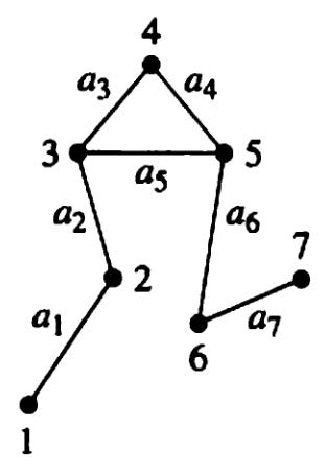
\includegraphics[width=0.15\textwidth]{HW10-1}
		\end{center}			
		\begin{enumerate}[a.]
			\item			
			Is the graph simple? If no, why not?
			\item
			Is the graph complete? If no, why not?
			\item
			Is the graph connected? If no, why not?
			\item
			Can you find two paths from 3 to 6? If yes, give both paths.
			\item
			Can you find a cycle? If yes, give one cycle.
			\item
			Can you find an edge whose removal will make the graph acyclic? If yes, give one edge.
			\item
			Can you find an edge whose removal will make the graph not connected? If yes, give one edge.
		\end{enumerate}
	
	
		\newpage
		\item ($7 \times 3$)
		Use the directed graph in the figure to answer the following questions.
		\begin{center}
			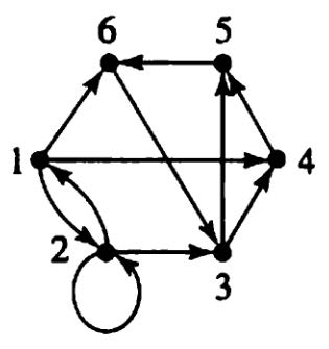
\includegraphics[width=0.15\textwidth]{HW10-2}
		\end{center}
		\begin{enumerate}[a.]
			\item 
			Which nodes are reachable from node 3?
			\item
			What is the length of the shortest path from node 3 to node 6?
			\item
			What is a path form node 1 to node 6 of length 8?
		\end{enumerate}
		

		

		

		
	\end{enumerate}
\end{document}
%==============================================================================
